							\chapter{Rocket Analysis}

		\section{Take into note that this is a not even a real draft}
		
		
		
		
	\section{ Rocket Description}

same as in chapter 5 for the inverted pendulum description
For this project a rocket is built. It consists of:
\begin{itemize}
\item a thruster
\item a sensor - gyroscope, blablabla
\item a controller - an arduino
\item a rocket body connected to the thruster with a liberty of movement of one degree
\end{itemize}

	\section{Inverted pendulum and rocket}
The goal of this section is to demonstrate the similarities between the inverted pendulum and the rocket stabilization processes, and to define a mathematical model and control loop of the behavior of the angle of the rocket body and the angle of the thruster.

The purpose of the system is to guarantee a stable flight to the rocket.
The modelling of the flight of a rocket can be divided into two equations: velocity and rotation. In this project, the desired trajectory of the rocket flight is considered to be on the zenith axis. This results in a vertical flight, with then a velocity on the same axis as the trajectory.The rocket's rotation is a circular motion on the bottom-to-nose axis. This create a centripetal force.

The displacement angle (gimbal angle) is the difference between the actual flight direction, or bottom-to-nose axis, and the zenith axis. Gimbaled thrust are controllable thrusters used to create a torque and reduce the gimbal angle. 

In an inverted pendulum, the objective is to keep the stick in horizontal position. The angle difference between the horizontal and the actual axis of the stick is measured in order to then create a compensation torque with the arm. The arm has the same task as the gimbaled thruster, and the horizontal axis is equivalent to the zenith axis.

At the desired initial position of the inverted pendulum, the acceleration of the arm is negligible. This implies that the arm only produces a force on the axis going through the center of gravity of the arm and parallel to the lenght of the arm. This is equivalent to the rocket process where the thruster applies a force on the axis going through the center of gravity of the arm and parallel to the lenght of the thruster. 

 Sketch of rocket + IP at initial position

Therefore the rocket and the inverted pendulum processes are equivalent for a small displacement angle range. The inverted pendulum is then studied in this project as a first approach to the understanding of rocket in-flight stabilization process.

The control loop of the rocket system is described in figure ...

Figure of closed loop model of rocket

The input of the closed loop is the gimbal angle (angle difference between actual flight direction and zenith axis). The output is the new gimbal angle. In the inverted pendulum, the input and output are also the angle differences, between the horizontal and the actual axis of the stick. 

By admiting that the inverted pendulum and the rocket processes are similar the equations found in Section 5.2 Modelling of the Arm and Stick can be applied to the rocket, with the rocket body as the stick and the gimbaled thruster as the arm. However the gravity center of the rocket body is not located in its center. Therefore $l_{a}$ and $\frac{l_{s}}{2}$ become respectively $l_{t}$, for the thruster, and $l_{bg}$, for the lenght from the bottom of the rocket body to its center of mass. The equations describing the forces, with $a$ for arm and $s$ for stick respectively replaced by $t$ for thruster and $b$ for rocket body, are:

Transfer function as in part "modeling of stick".

	\section{Modeling of the rocket body and stick}
	
The purpose of this section is to have a mathematical model for the different forces applied on the rocket in flight. 

In this project, the trajectory of the rocket is on the zenith axis, or y axis, which implies the impact of the lift on the rocket is negligible. The sum of the forces applied to the rocket in flight can then be described by equation \eqref{eq:F_total}:

\begin{equation}
F_{total} = m*a = F_{thrust} + F_{drag} - F_{gravity} \si{\newton} \label{eq:F_{total}}
\end{equation}
\startexplain
\explain{$F_{total}$ is the sum of all force}{\si{\newton}}
\explain{$F_{thrust}$ is the force created by the gimbaled thruster}{\si{\newton}}
\explain{$F_{drag}$ is the drag force on the rocket}{\si{\newton}}
\explain{$F_{gravity}$ is the gravity applied on the rocket}{\si{\newton}}
\stopexplain

The drag force can be expressed by equation \eqref{eq:F_drag}:
\begin{equation}
F_{drag} = \frac{1}{2} \cdot C_{d} \cdot \rho \cdot A \cdot v^2 \si{\newton} \label{eq:F_{drag}}
\end{equation}
\startexplain
\explain{$C_{d}$ is the coefficient of drag}{\si{1}}
\explain{$\rho$ is the air density}{\si{\kilo\gram\per\meter\cubed}}
\explain{$A$ is the cross sectionnal area of the rocket}{\si{\meter\squared}}
\explain{$v$ is the velocity of the rocket}{\si{\meter\per\second}}
\stopexplain
	
The coefficient of drag and the cross sectionnal area vary depending on the shape of the rocket. Altitude and humidity in the air can impact the air density. Parasit drag can appear due to the surface material or pressure drag.

The gravity force equation is \eqref{eq:F_{gravity}}:
\begin{equation}
F_{gravity} = m \cdot g \si{\newton} \label{eq:F_{gravity}}
\end{equation}
\startexplain
\explain{$m$ is the mass of the rocket}{\si{\kilo\gram}}
\explain{$g$ is the gravitational acceleration}{\si{\meter\per\second\squared}}
\explain{$A$ is the cross sectionnal area of the rocket}{\si{\meter\squared}}
\explain{$v$ is the velocity of the rocket}{\si{\meter\per\second}}
\stopexplain
	

The thrust force is \eqref{eq:F_{thrust}}:
\begin{equation}
F_{thrust} = v_{e} \cdot \ddot{m} + A (P_{e} -P_{0}) \si{\newton} \label{eq:F_{thrust}}
\end{equation}
\startexplain
\explain{$v_{e}$ is the velocity of the gimbaled thruster}{\si{\meter\per\second}}
\explain{$\ddot{m}$ is the mass flow rate}{\si{\kilo\gram\per\second}}
\explain{$A$ is the nozzle exit area}{\si{\meter\squared}}
\explain{$P_{e}$ is the pressure of the nozzle exit}{\si{\kilo\gram\per\meter\per\second\squared}}
\explain{$P_{0}$ is the free stream pressure}{\si{\kilo\gram\per\meter\per\second\squared}}
\stopexplain


The thruster pression and velocity is divided into two equation, respectively ahead and behind the propeller nozzle: $P_{o}$ \eqref{eq:P_{o}} and $P_{e}$ \eqref{eq:P_{e}}.

\begin{equation}
P_{0} = p_{0} + 0.5 \cdot \rho \cdot(v_{o})^2 \si{\kilo\gram\per\meter\per\second\squared} \label{eq:P_{o}}
\end{equation}
\startexplain
\explain{$p_{o}$ is the static pressure}{\si{\kilo\gram\per\meter\per\second\squared}}
\explain{$v_{o}$ is the velocity of the rocket}{\si{\meter\per\second}}
\stopexplain

\begin{equation}
P_{e} = p_{o} + 0.5 \cdot \rho \cdot(v_{e})^2 \si{\kilo\gram\per\meter\per\second\squared} \label{eq:P_{e}}
\end{equation}
\startexplain
\explain{$v_{e}$ is the exit velocity of the gimbaled thruster}{\si{\meter\per\second}}
\stopexplain

Therefore, there is three different cases of truster pression:
\begin{equation}
P_{e} = P_{a}
P_{e} > P_{a}
P_{e} < P_{a}
\end{equation}
 insert sketch of the different cases
 
 
 
 
 
 
 

		\section{This is the modified version of the Inverted Pendulum Analysis}
		
		
		
		
\section{Inverted Pendulum Description}
For this project an inverted pendulum set up is given. It consists of:
\begin{itemize}
	\item A DC motor
	\item A gear system
	\item An arm
	\item A stick connected to the end of the arm.
\end{itemize}

\begin{figure} [htbp]
	\centering
	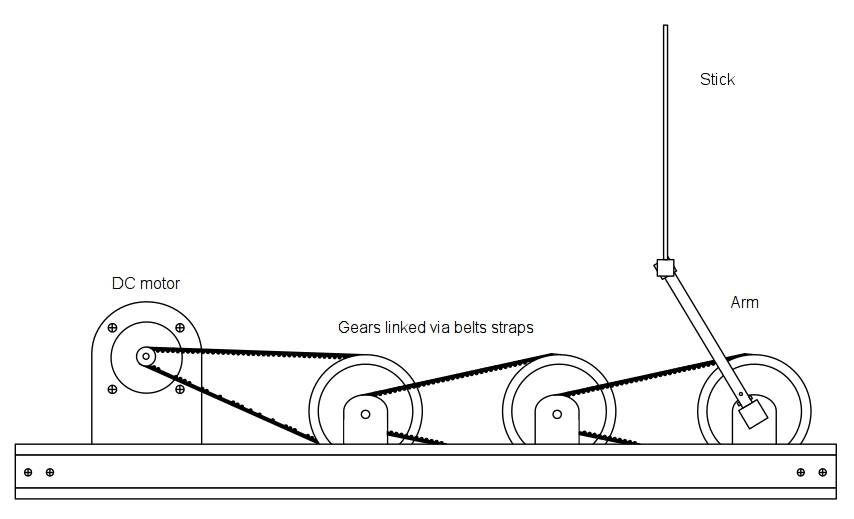
\includegraphics[width=0.6\linewidth]{figures/"Preanalysis&Requirement"/invertedPendulumDiagram}
	\caption{Diagram of the set up fully assembled} \label{fig:InvertedPendulumSetUp}
\end{figure}

\autoref{fig:InvertedPendulumSetUp} is a diagram of the set up when fully assembled. The DC motor moves the arm via the gears, a noteworthy fact is that out the four gears three are of the same size. This means that two gears do not have any influence on the torque and the angular velocity of the arm.

\section{Inverted Pendulum Hardware}
The following section describes the hardware connected to the inverted pendulum setup illustrated cf. figure \ref{fig:InvertedPendulumSetUp}.
Each part will be described with its specifications and use in the setup.

\subsubsection{Stick and Arm}
The arm and stick is elements that always appears in the double inverted pendulum setup. The goal is for the arm to apply force on the joint, which would affect the position of the stick. 

Stick length: 80 cm
Stick weight: 344 grams

Stick length: 40 cm
Stick weight: 170 grams
 
Arm length: 33 cm
Arm weight: 288 grams

\subsubsection{DC Motor}
Alsthom BBC MODEL: F9M2 AAU:08339
\ref{appendix:DCMotorInductance}

\subsubsection{Gear System}
Gear teeth big: 40
Gear teeth small: 12
Belt length: 60 cm
Wheel diameter big: 12 cm
Wheel diameter small: 4 cm


\section{Modelling of the Arm and Stick}\label{sec:StickArm}

%%%%%%%%%%%%% Equation template %%%%%%%%%%%%%%%
%\begin{flalign}
%\hspace{30pt} & EQUATION1 &&& \text{[UNIT]} \notag \\
%& EQUATION2 &&& \text{[UNIT]} \label{eq:LABEL} 
%\end{flalign}
%\begin{description}
%  \item[\hspace{30pt}\textnormal{where:}]\hfill \\
%  \begin{tabular}{p{30pt}lp{250pt}l}
%& $x$ & TEXT & [UNIT]  \\
%& $y$ & VERY LONG TEXT THAT IS VERY LONG AND HAS A LOT OF WORDS IN IT YET THE FORMATTING STILL LOOKS NICE AND CLEAN AND EVERYTHING IS AWESOME & [UNIT]  \\
%& $z$ & TEXT & [UNIT]
%\end{tabular}
%\end{description}
%%%%%%%%%%%%%%%%%%%%%%%%%%%%%%%%%%%%%%%%%%%%%%%
\graphicspath{{figures/Preanalysis&Requirement/PendulumModeling/}}
The goal of this section is to have a mathematical model for the behavior of the angle of the stick in relation to the angle of the arm on the motor. The angles, constants and forces used to describe the system are seen on \autoref{fig:ArmStick}.
%\todo[inline,author=Jacob]{I'd like to somehow describe the process first instead of just going along randomly and suddenly ending up with the model. "We want to achieve this so we do that" etc.}
\begin{figure}[htbp]
	\centering
	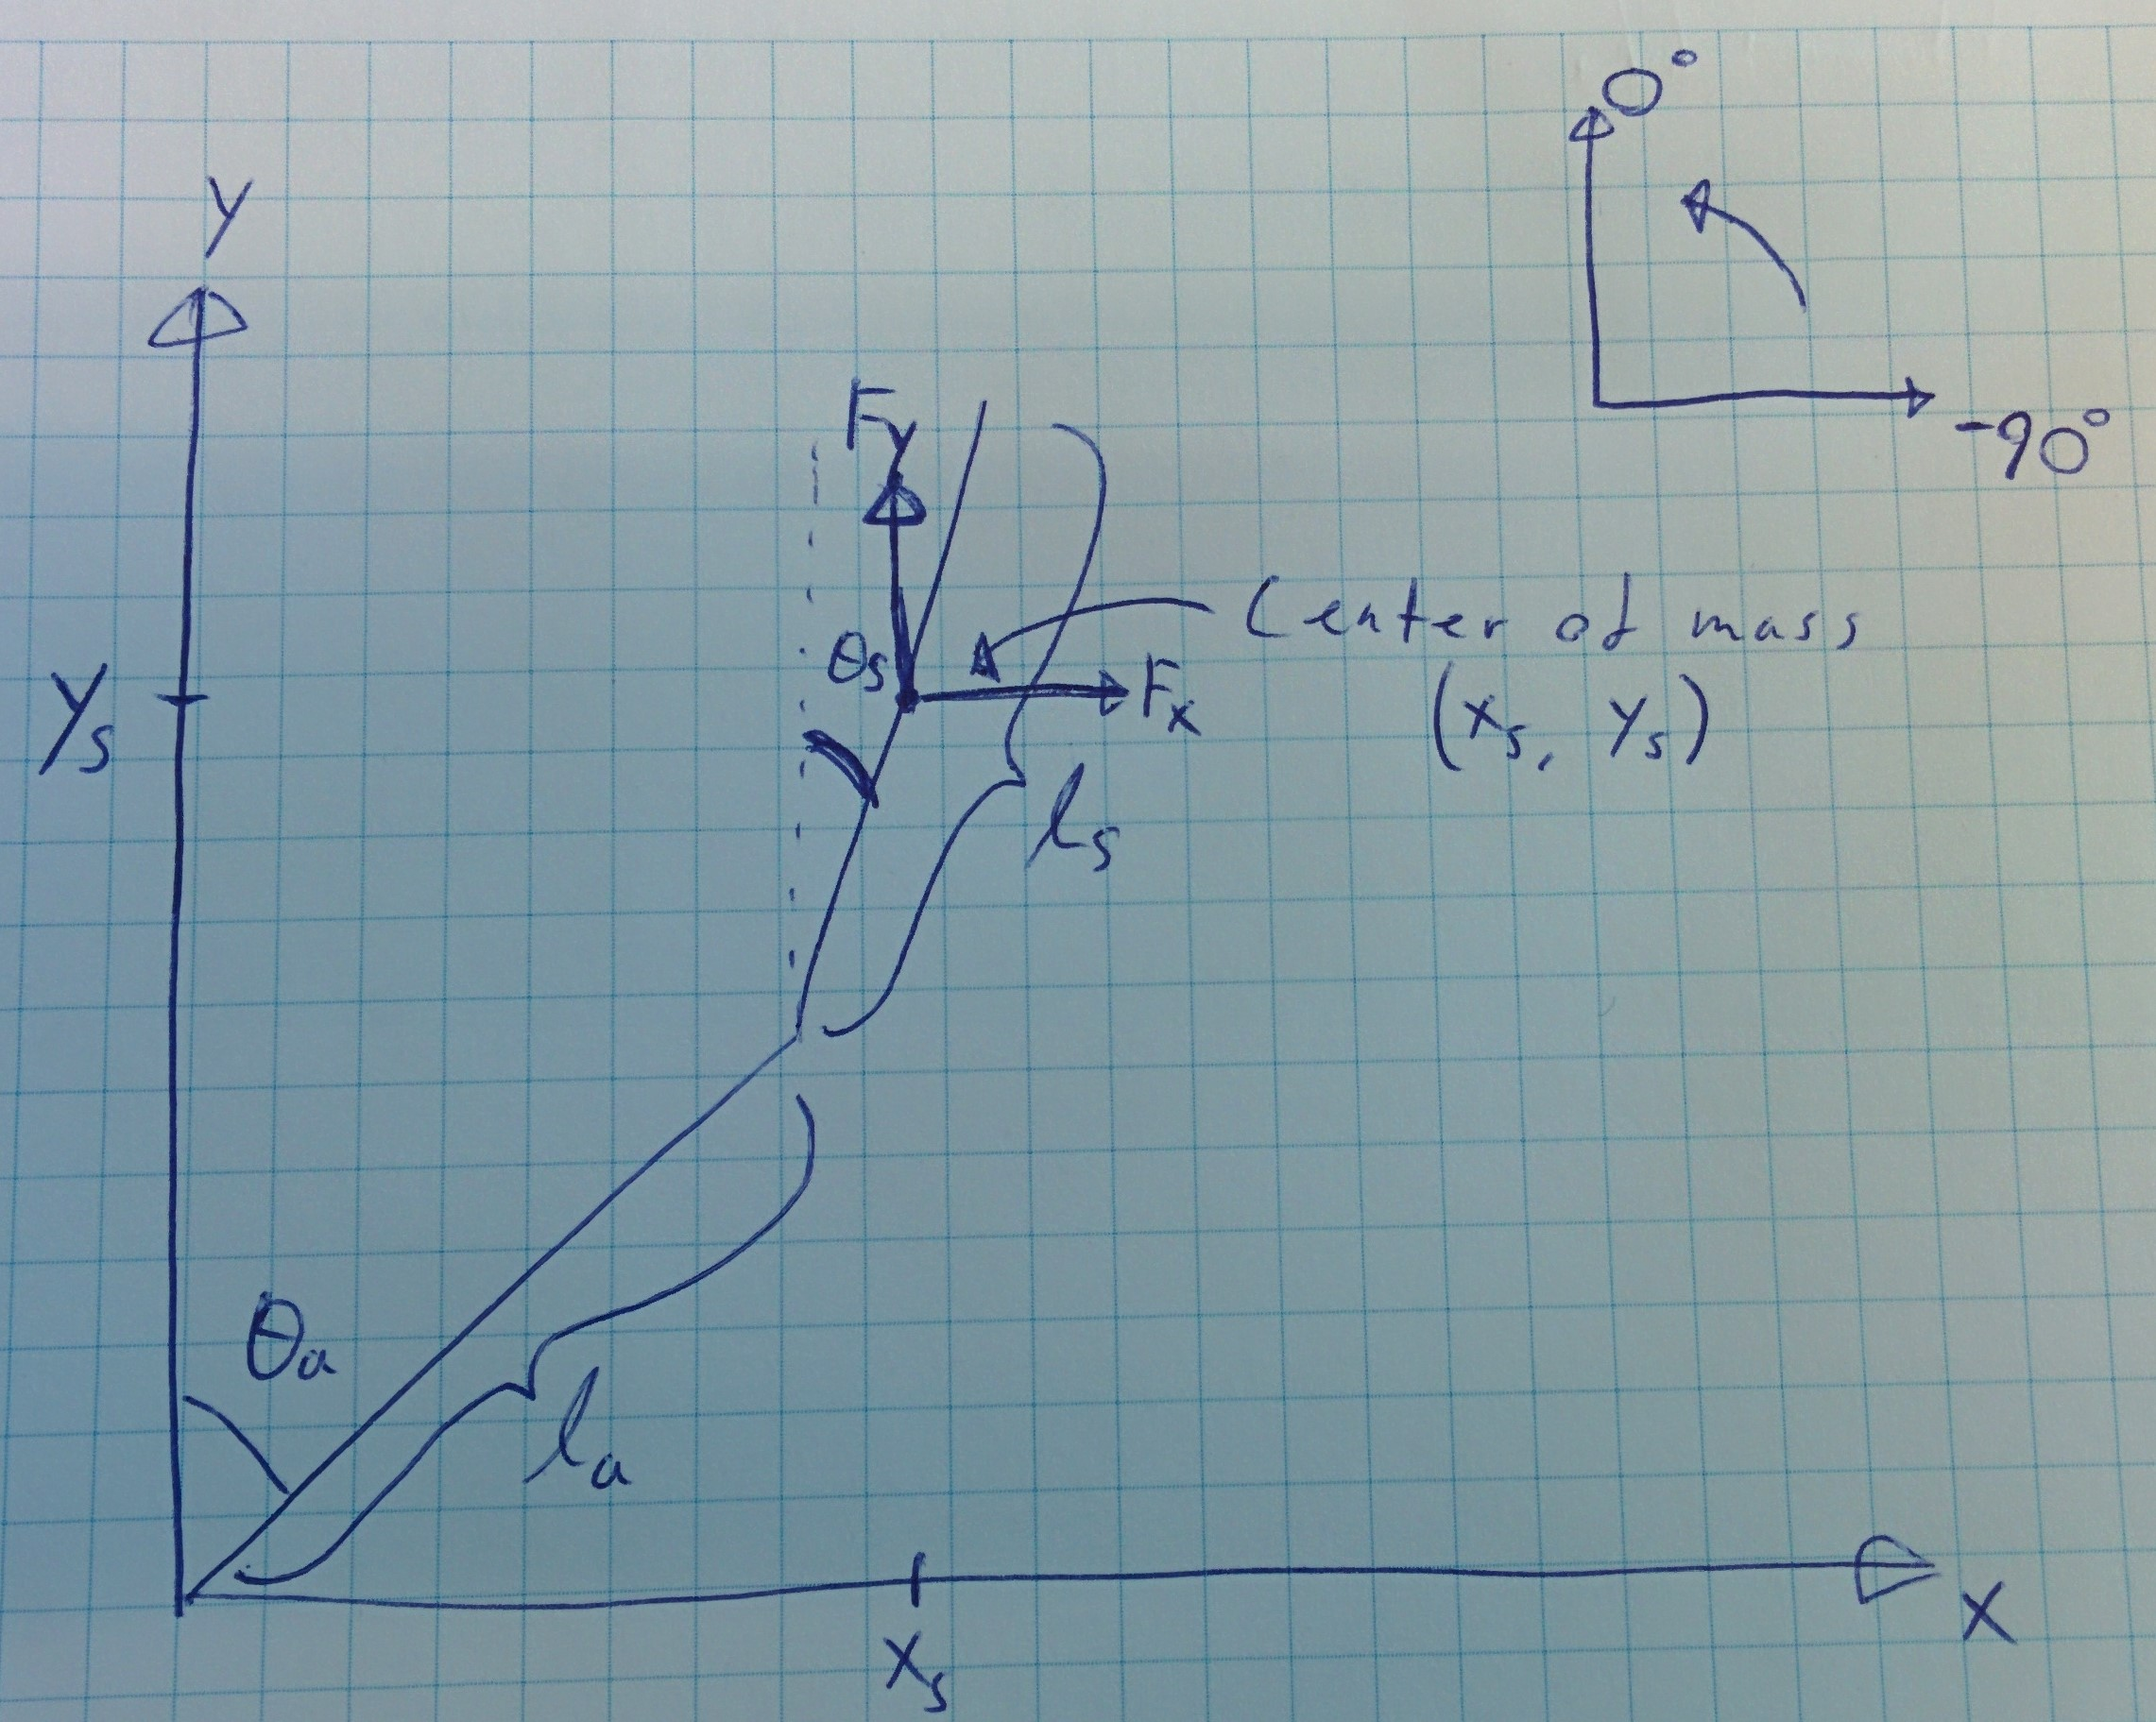
\includegraphics[width=0.8\textwidth]{StickAndForces}
	\caption{Diagram of the angles and forces acting on the arm and the stick.}
	\label{fig:ArmStick}
\end{figure}

\startexplain
\explain{$F_x$ is the force in the x direction}{\si{\newton}}
\explain{$F_y$ is the force in the y direction}{\si{\newton}}
\explain{$x_s$ is the position of the center of mass of the stick in the x direction}{\si{\meter}}
\explain{$y_s$ is the position of the center of mass of the stick in the y direction}{\si{\meter}}
\explain{$l_a$ is the length of the arm}{\si{\meter}}
\explain{$l_s$ is the length of the stick}{\si{\meter}}
\explain{$\theta_a$ is the angle from the arm to the y-axis}{\si{\radian}}
\explain{$\theta_s$ is the angle from the stick to the y-axis}{\si{\radian}}
\stopexplain
All forces, constants and variables that relates to the arm and stick are denoted by a subscripted $a$ and $s$ respectively. 

The behaviour of the stick can be fully described by three movements; two translatory and one rotary. It can move in the x and y direction and rotate around it's own axis.

%To find the relation between the angles, the free body diagram of the joint of the arm and stick is made on \autoref{fig:freebodystick}.
%\begin{figure}[htbp]
%\centering
%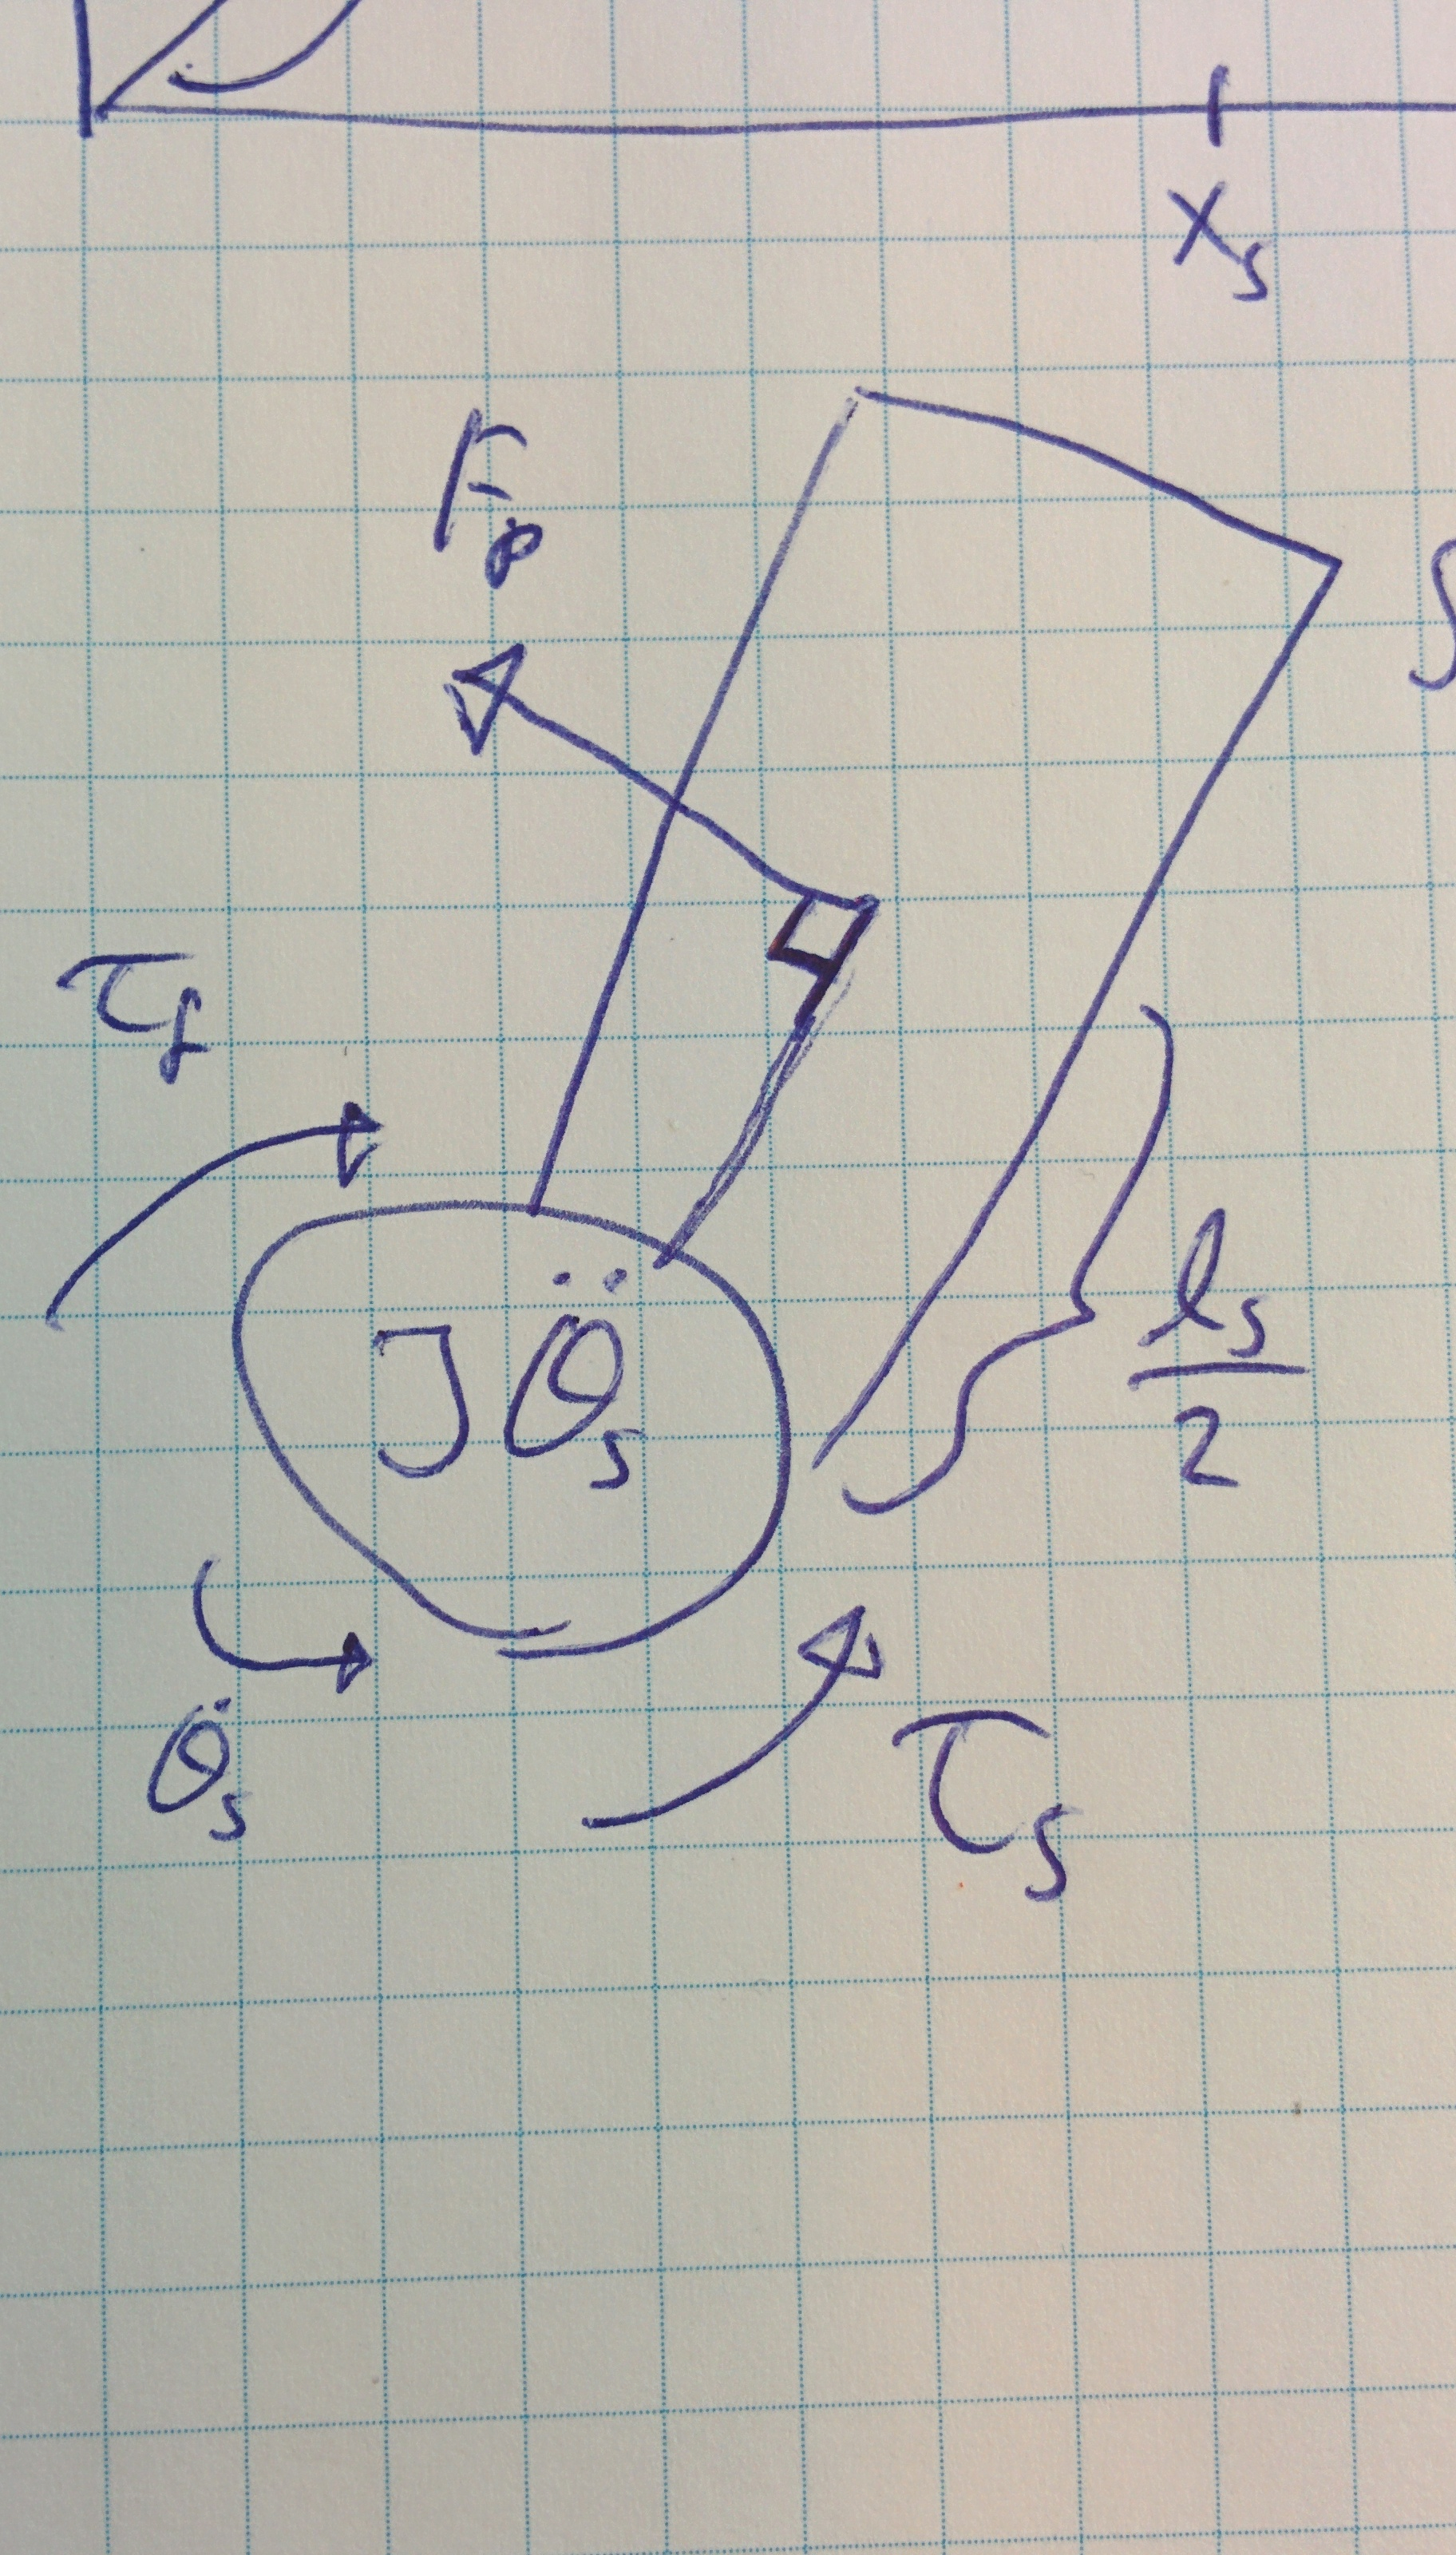
\includegraphics[width=0.25\textwidth]{FreeBodyPendulum}
%\caption{Free body diagram of the joint that connects the arm and the stick.}
%\label{fig:freebodystick}
%\end{figure}
%\todo[inline, author=Jacob]{Make pretty graph}
%
%The moment of inertia for the joint is described by \autoref{eq:Jsthetas}.
%\begin{subequations}
%\begin{flalign}
%& J_s\ddot{\theta}_s=\tau_s-\tau_f  \label{eq:Jsthetas} \\
%& \tau_s =F_p\frac{l_s}{2} \\
%& \tau_f =b_{as}\dot{\theta}_{as} 
%\end{flalign}
%\end{subequations}
%\startexplain
%	\explain{$J_s$ is the moment of inertia for the stick}{\si{\kg\square\meter}}
%	\explain{$\ddot{\theta}_s$ is the angular acceleration of the stick}{\si{\radian\per\square\second}}
%	\explain{$\tau_s$ is the torque induced by the rotation of the stick}{\si{\newton\meter}}
%	\explain{$\tau_f$ is the torque of the friction acting on the stick}{\si{\newton\meter}}
%	\explain{$F_p$ is the force perpendicular to the stick at the center of mass}{\si{\newton}}
%	\explain{$b_{as}$ is the viscous friction coefficient between the arm and the stick}{\si{\newton\meter\second}}
%	\explain{$\dot{\theta}_{as}$ is the difference in angular velocity between the arm and the stick ($\dot{\theta}_s-\dot{\theta}_a$)}{\si{\radian\per\second}}
%\stopexplain
%
%The friction is calculated from the difference in angular velocity as the stick could be perfectly upright while the arm moves causing the joint to turn. The angle of the arm is not considered as producing a torque acting on the joint but as part of the force on the stick, $F_p$.

The forces acting on the stick in the x and y directions are found by \autoref{eq:FxFy} using Newton's 2nd law of motion.
\begin{subequations}  \label{eq:FxFy}
	\begin{flalign}
		& F_x=\ddot{x}_sM_s  \\
		& F_y-gM_s=\ddot{y}_sM_s  \\
		& F_y=\left(\ddot{y}_s+g\right)M_s
	\end{flalign}
\end{subequations}
\startexplain
\explain{$g$ is the standard gravitational acceleration near the surface of the earth}{\si{\meter\per\square\second}}
\explain{$M_s$ is the mass of the stick}{\si{\kilo\gram}}
\stopexplain
The position of the center of mass of the stick in the x and y direction is found by \autoref{eq:xsys} using geometry.
\begin{subequations}\label{eq:xsys} 
	\begin{flalign}
		& x_s=l_a\sin (-\theta_a)+\frac{l_s}{2} \sin (-\theta_s) \\
		& x_s=-l_a\sin (\theta_a)-\frac{l_s}{2} \sin (\theta_s) \\
		& y_s = l_a\cos (-\theta_a)+\frac{l_s}{2} \cos(-\theta_s) \\
		& y_s = l_a\cos (\theta_a)+\frac{l_s}{2} \cos(\theta_s) 
	\end{flalign}
\end{subequations}

The derivatives of $x_s$ and $y_s$ is found in \autoref{eq:diffxy}.
\begin{subequations}\label{eq:diffxy} 
	\begin{flalign}
		\hspace{30pt} & \dot{x}_s=-l_a\dot{\theta}_a\cos(\theta_a)-\frac{l_s}{2}\dot{\theta}_s\cos(\theta_s) & [\si{\meter\per\second}] \\
		& \ddot{x}_s=-l_a\ddot{\theta}_a\cos(\theta_a)+l_a\dot{\theta}_a^2\sin(\theta_a)-\frac{l_s}{2}\ddot{\theta}_s\cos(\theta_s)+\frac{l_s}{2}\dot{\theta}_s^2\sin(\theta_s) & [\si{\meter\per\square\second}] \\
		& \dot{y}_s=-l_a \dot{\theta}_a\sin(\theta_a)-\frac{l_s}{2}\dot{\theta}_s\sin(\theta_s) & [\si{\meter\per\second}] \\
		& \ddot{y}_s=-l_a\ddot{\theta}_a\sin(\theta_a)-l_a\dot{\theta}_a^2\cos(\theta_a)-\frac{l_s}{2}\ddot{\theta}_s\sin(\theta_s)-\frac{l_s}{2}\dot{\theta}_s^2\cos(\theta_s) & [\si{\meter\per\square\second}]
	\end{flalign}
\end{subequations}

The forces $F_x$ and $F_y$ can be decomposed into perpendicular and parallel forces at that point. The parallel forces are negligible when assuming the stick is perfectly solid and unable to stretch or compress. The perpendicular forces is found by \autoref{eq:perpFxFy} and are seen on \autoref{fig:ArmStick}.

%\begin{figure}[htbp]
%\centering
%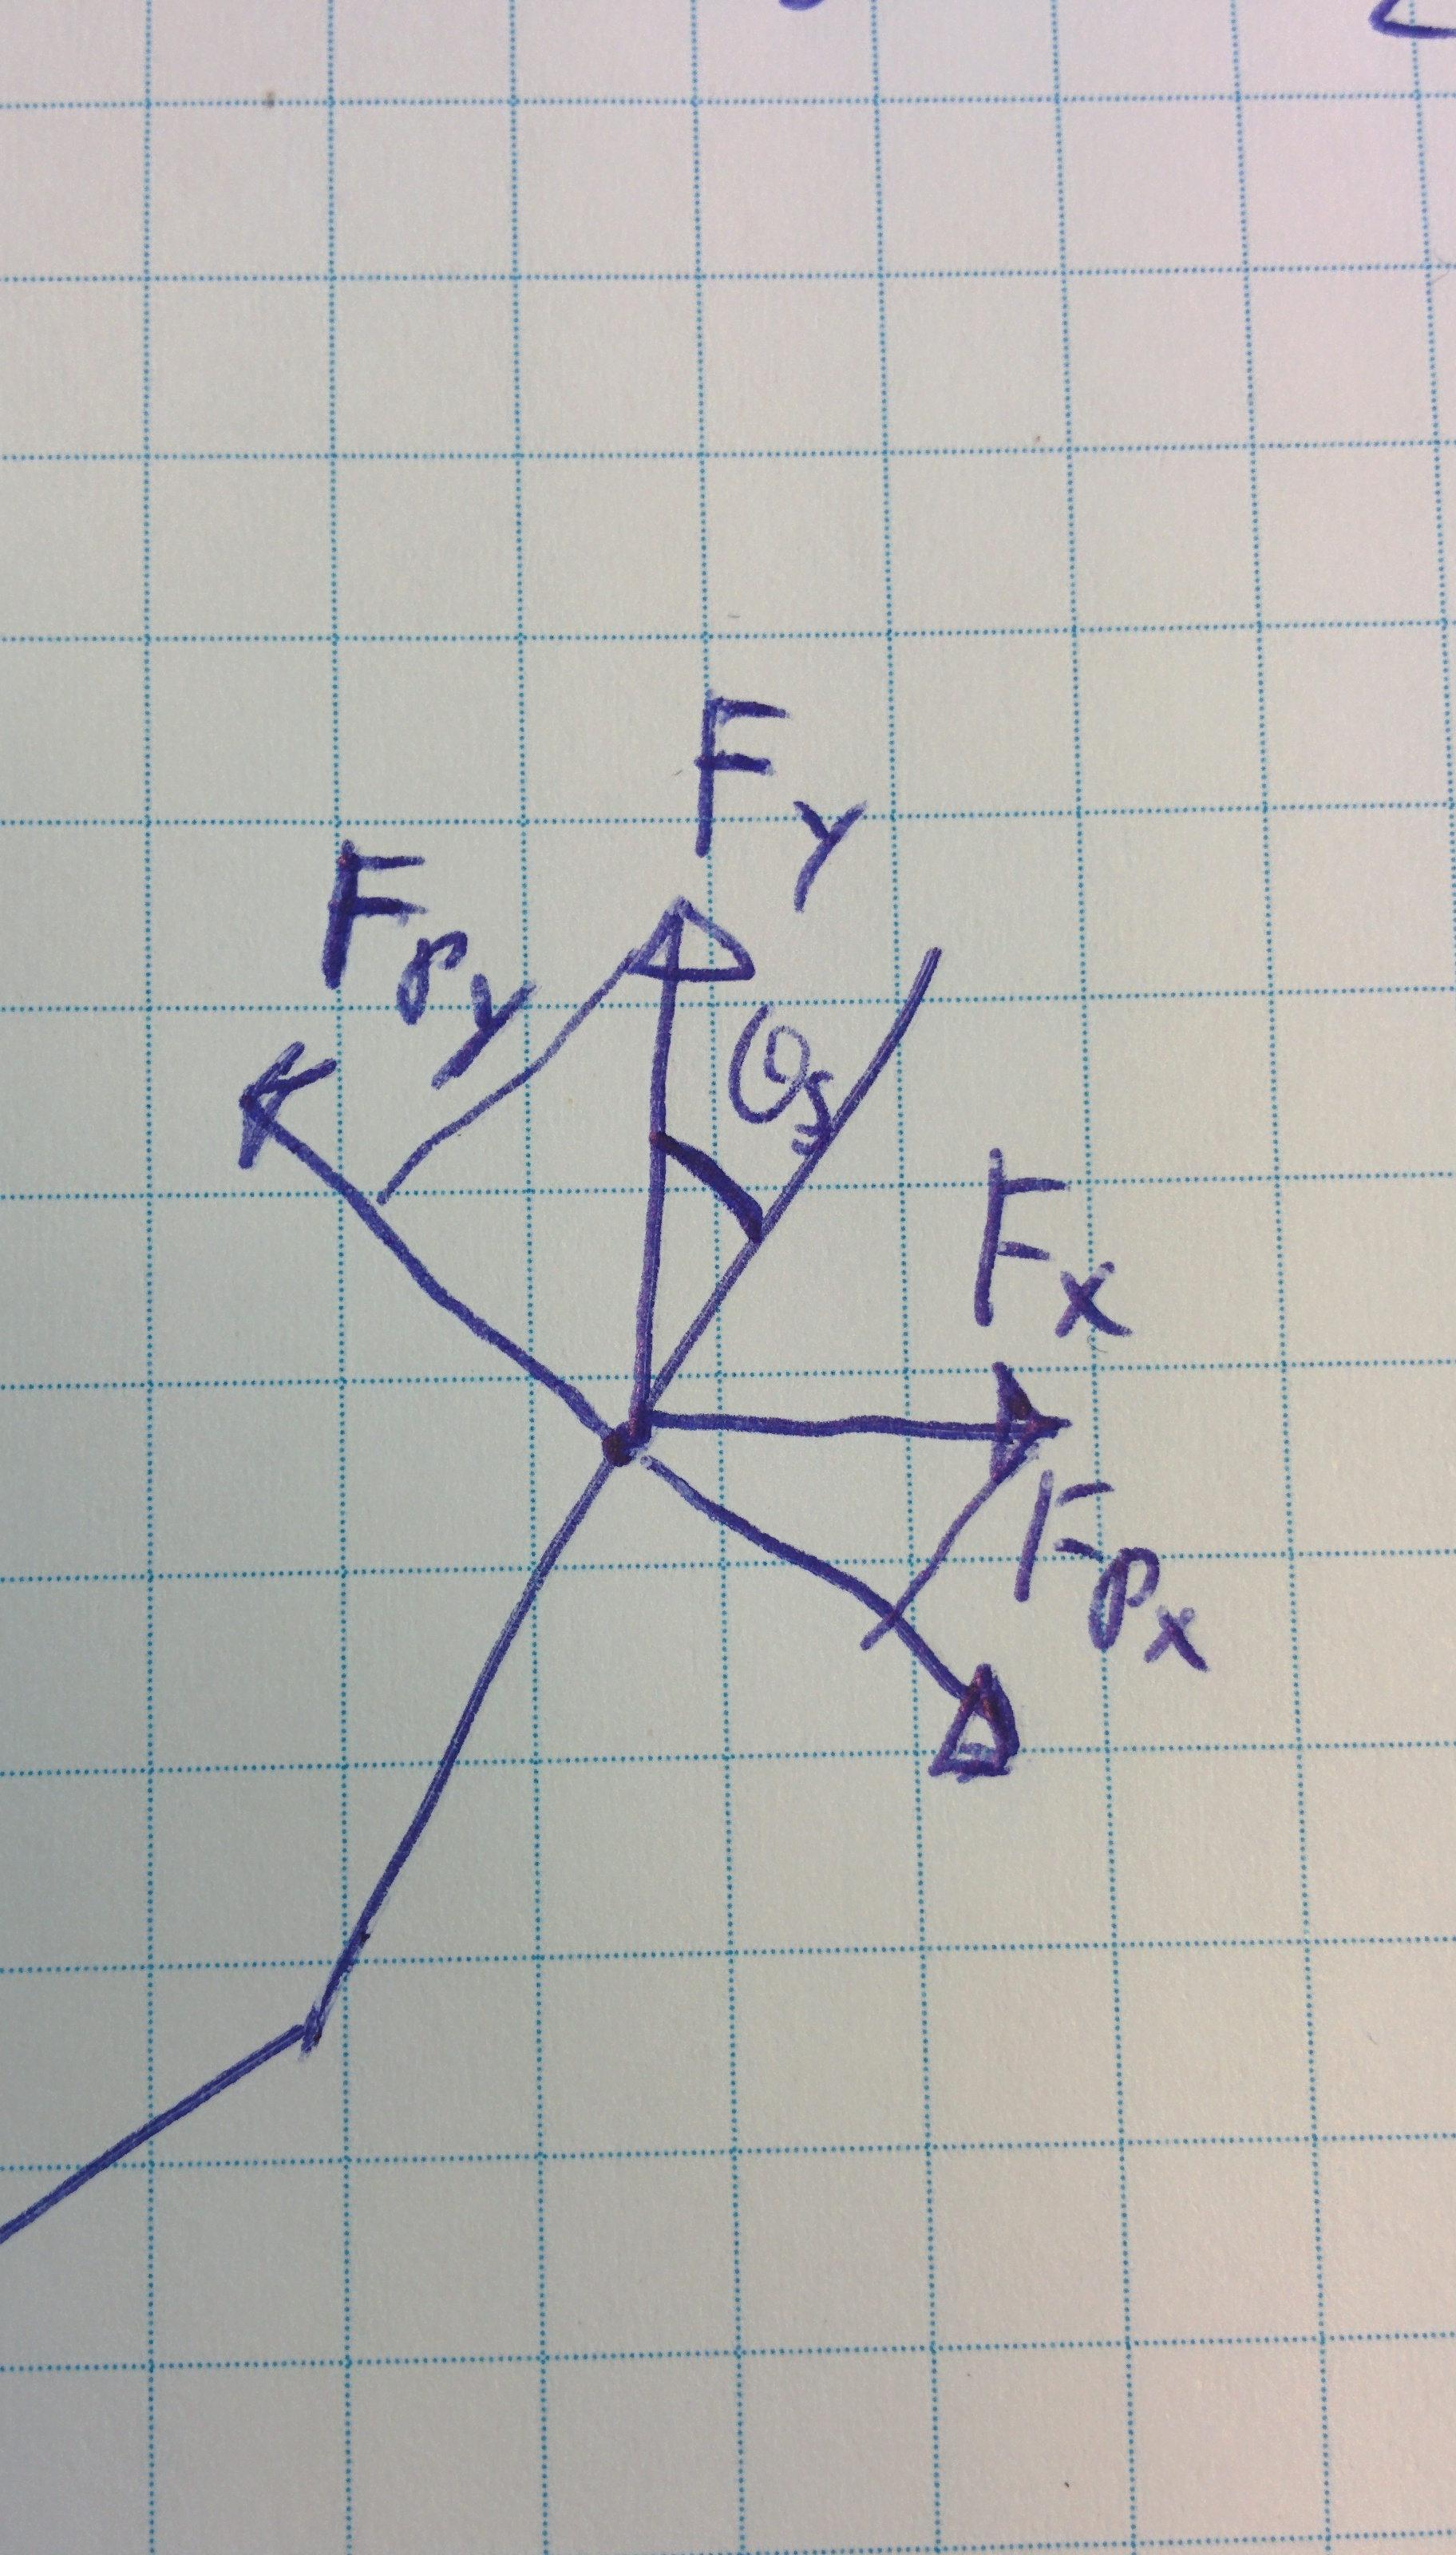
\includegraphics[width=0.25\textwidth]{ForcePerp}
%\caption{Diagram of the forces, $F_x$ and $F_y$, decomposed into perpendicular forces.}
%\label{fig:ForcePerp}
%\end{figure}

\begin{subequations}\label{eq:perpFxFy}
	\begin{flalign}
		& F_{px}=F_x\cos(\theta_s) \\
		& F_{py}=F_y\sin(\theta_s)  \\
		& F_p = F_{px}+F_{py} 
	\end{flalign}
\end{subequations}

The rotary force of the stick is described by \autoref{eq:JsLong}.
\begin{subequations}
	\begin{flalign}
		J_s\ddot{\theta}_s &=\frac{l_s}{2}\left(F_x\cos(\theta_s)+F_y\sin(\theta_s)\right)-b_{as}\dot{\theta}_{as}  \\
		J_s\ddot{\theta}_s = \frac{l_s}{2}M_s \Big( &-l_a\ddot{\theta}_a\left(\cos(\theta_a)\cos(\theta_s)+\sin(\theta_a)\sin(\theta_s)\right) \notag \\
		& +l_a\dot{\theta}_a^2\left(\sin(\theta_a)\cos(\theta_s)-\cos(\theta_a)\sin(\theta_s)\right) \notag \\
		& -\frac{l_s}{2}\ddot{\theta}_s\left(\cos(\theta_s)\cos(\theta_s)+\sin(\theta_s)\sin(\theta_s)\right) \notag \\
		& +\frac{l_s}{2}\dot{\theta}_s^2\left(\sin(\theta_s)\cos(\theta_s)-\cos(\theta_s)\sin(\theta_s)\right)  \notag \\
		& +g\sin(\theta_s) \Big)-b_{as}\dot{\theta}_{as} \label{eq:JsLong}
	\end{flalign}
\end{subequations}

Using the trigonometric properties in \autoref{eq:trigprop}, \autoref{eq:JsLong} is reduced to \autoref{eq:JsShort}.
\begin{subequations} \label{eq:trigprop}
	\begin{flalign}
		& \cos(\theta_a)\cos(\theta_s)\pm \sin(\theta_a)\sin(\theta_s)=\cos(\theta_a \mp \theta_s)  \\
		& \sin(\theta_a)\cos(\theta_s)\pm \cos(\theta_a)\sin(\theta_s) = \sin(\theta_a \pm \theta_s) \\ 
		& \cos(\theta_s)^2+\sin(\theta_s)^2=1 
	\end{flalign}
\end{subequations}
\begin{flalign}
	J_s\ddot{\theta}_s = \frac{l_s}{2}M_s \Big( &-l_a\ddot{\theta}_a \cos(\theta_a-\theta_s)+l_a\dot{\theta}_a^2 \sin(\theta_a-\theta_s) \notag \\
	&-\frac{l_s}{2}\ddot{\theta}_s +g\sin(\theta_s) \Big)-b_{as}\dot{\theta}_{as} \label{eq:JsShort}
\end{flalign}

This is the nonlinear mathematical model for the system. This will be linearized in order to perform a Laplace transformation. The linearization is made with a 1st order Taylor approximation. The linearization is done at the equilibrium point where the arm is in an upright position i.e. $\theta_s=0$. In the equilibrium point the derivatives of all the inputs and outputs are 0. In this case the inputs and outputs are $\theta_a$ and $\theta_s$ and the operating point is $\bar{\theta}_a=0$ and $\bar{\theta}_s=0$. The nonlinear model is expressed as a function of the inputs and outputs as seen in \autoref{eq:nonlinearmodel}.
\begin{flalign}\label{eq:nonlinearmodel}
	f\left(\theta_a, \dot{\theta}_a, \ddot{\theta}_a, \theta_s, \ddot{\theta}_s\right)=\frac{l_s}{2}M_s \Big( &-l_a\ddot{\theta}_a \cos(\theta_a-\theta_s)+l_a\dot{\theta}_a^2 \sin(\theta_a-\theta_s) \notag \\
	&-\frac{l_s}{2}\ddot{\theta}_s +g\sin(\theta_s) \Big)-b_{as}\dot{\theta}_{as}-J_s\ddot{\theta}_s
\end{flalign}

Generally all equilibriums can be found by setting \autoref{eq:nonlinearmodel} equal to 0 and the derivatives to 0 and solving for $\theta_a=\bar{\theta}_a$ and $\theta_s=\bar{\theta}_s$. For the pendulum it's easy to see the only two equilibriums are the stick pointing straight up and straight down. 

The 1st order Taylor approximation of an equation with multiple variables is seen in \autoref{eq:1stTaylor}.
\begin{flalign}
	f\left(\theta_a, \dot{\theta}_a, \ddot{\theta}_a, \theta_s, \ddot{\theta}_s\right) & \approx f\left(\bar{\theta}_a, 0, 0, \bar{\theta}_s, 0\right) + \left. \frac{\partial f}{\partial \theta_a}\right|_{(\bar{\theta}_a, \bar{\theta}_s)} \hat{\theta}_a \notag \\
	& \phantom{=} + \left. \frac{\partial f}{\partial \dot{\theta}_a}\right|_{(\bar{\theta}_a, \bar{\theta}_s)} \hat{\dot{\theta}}_a + \left. \frac{\partial f}{\partial \ddot{\theta}_a}\right|_{(\bar{\theta}_a, \bar{\theta}_s)} \hat{\ddot{\theta}}_a \notag \\
	& \phantom{=} + \left. \frac{\partial f}{\partial \theta_s}\right|_{(\bar{\theta}_a, \bar{\theta}_s)} \hat{\theta}_s + \left. \frac{\partial f}{\partial \ddot{\theta}_s}\right|_{(\bar{\theta}_a, \bar{\theta}_s)} \hat{\ddot{\theta}}_s \label{eq:1stTaylor}
\end{flalign}
\startexplain
\explain{$\bar{\theta}$ denotes the angle in an operating point}{\si{\radian}}
\explain{$\hat{\theta}$ denotes the angle of the small signal variances}{\si{\radian}}
\stopexplain

The 3 terms with sin or cos in \autoref{eq:JsShort} will be approximated individually using \autoref{eq:1stTaylor}, remembering that $\bar{\theta}=\bar{\dot{\theta}}=\bar{\ddot{\theta}}=0$ in the equilibrium.
\begin{subequations}
	\begin{flalign}
		-l_a\ddot{\theta}_a\cos\left(\theta_a-\theta_s\right)  \approx & \ 0 + l_a\bar{\ddot{\theta}}_a\sin\left(\bar{\theta}_a-\bar{\theta}_s\right)\hat{\theta}_a  \notag \\ 
		& -l_a\cos\left(\bar{\theta}_a-\bar{\theta}_s\right)\hat{\ddot{\theta}}_a - l_a\bar{\ddot{\theta}}_a\sin\left(\bar{\theta}_a-\bar{\theta}_s\right)\hat{\theta}_s   \\
		-l_a\ddot{\theta}_a\cos\left(\theta_a-\theta_s\right) \approx &-l_a\hat{\ddot{\theta}}_a 
	\end{flalign} %\bar{\ddot{\theta}}_s
\end{subequations}
\begin{subequations}
	\begin{flalign}
		l_a\dot{\theta}_a^2\sin\left(\theta_a-\theta_s\right)  \approx &\ 0 + l_a\bar{\dot{\theta}}_a^2\cos\left(\bar{\theta}_a-\bar{\theta}_s\right)\hat{\theta}_a  \notag \\
		& + 2l_a\bar{\dot{\theta}}_a\sin\left(\bar{\theta}_a-\bar{\theta}_s\right)\hat{\dot{\theta}}_a-l_a\bar{\dot{\theta}}_a^2\cos\left(\bar{\theta}_a-\bar{\theta}_s\right)\hat{\theta}_s   \\
		l_a\dot{\theta}_a^2\sin\left(\bar{\theta}_a-\bar{\theta}_s\right) \approx & \ 0 
	\end{flalign}
\end{subequations}
\begin{subequations}
	\begin{flalign}
		& g\sin\left(\theta_s\right) \approx g\sin\left(\bar{\theta}_s\right) +g\cos\left(\bar{\theta}_s\right)\hat{\theta}_s \\
		& g\sin\left(\theta_s\right) \approx g\hat{\theta}_s 
	\end{flalign}
\end{subequations}

Inserting the linearized terms in \autoref{eq:JsShort} and using the moment of inertia for a rotating stick, $J_s=\frac{1}{12}M_sl_s^2$, the linearized model becomes \eqref{eq:JsFinal}.
\begin{subequations}
	\begin{flalign}
		& \frac{1}{12}M_sl_s^2\hat{\ddot{\theta}}_s=\frac{l_s}{2}M_s\left(-l_a\hat{\ddot{\theta}}_a-\frac{l_s}{2}\hat{\ddot{\theta}}_s+g\hat{\theta}_s\right)-b_{as}\hat{\dot{\theta}}_{as}   \\
		& \frac{1}{12}M_sl_s^2\hat{\ddot{\theta}}_s+\frac{1}{4}M_sl_s^2\hat{\ddot{\theta}}_s=\frac{l_s}{2}M_s\left(-l_a\hat{\ddot{\theta}}_a+g\hat{\theta}_s\right)-b_{as}\hat{\dot{\theta}}_{as}   \\
		& \frac{1}{3}M_sl_s^2\hat{\ddot{\theta}}_s=\frac{l_s}{2}M_s\left(-l_a\hat{\ddot{\theta}}_a+g\hat{\theta}_s\right)-b_{as}\hat{\dot{\theta}}_{as}  \label{eq:TauSmLin} \\
		& \hat{\ddot{\theta}}_s=\frac{3}{2l_s}\left(-l_a\hat{\ddot{\theta}}_a+g\hat{\theta}_s\right)-\frac{3b_{as}\left(\hat{\dot{\theta}}_s-\hat{\dot{\theta}}_a\right)}{M_sl_s^2} \label{eq:JsFinal}
	\end{flalign}
\end{subequations}

The linearized model is now Laplace transformed in \autoref{eq:tfArmStick} in order to find the transfer function.
\begin{subequations}
	\begin{flalign}
		& s^2\Theta_s=\frac{3}{2l_s}\left(-s^2l_a\Theta_a+g\Theta_s\right)-s\frac{3b_{as}}{M_sl_s^2}\Theta_s+s\frac{3b_{as}}{M_sl_s^2}\Theta_a  \\
		& \Theta_s\left(s^2+\frac{3b_{as}}{M_sl_s^2}s-\frac{3g}{2l_s}\right)=\Theta_a\left(-\frac{3l_a}{2l_s}s^2+\frac{3b_{as}}{M_sl_s^2}s\right)  \\
		& \frac{\Theta_s}{\Theta_a}=-\frac{\frac{3l_a}{2l_s}s^2-\frac{3b_{as}}{M_sl_s^2}s}{s^2+\frac{3b_{as}}{M_sl_s^2}s-\frac{3g}{2l_s}} \label{eq:tfArmStick}
	\end{flalign}
\end{subequations}

A linearized model in the Laplace domain for the arm and the stick has been derived and the model for the gears is now derived.



